\documentclass{minimal}
\usepackage{tikz}
\usepackage{verbatim}
\usetikzlibrary{calc, trees, positioning, arrows, chains, matrix, shapes.geometric}

\usepackage{etoolbox}
%\pretocmd\tkzCircumCenter{\begin{pgfinterruptboundingbox}}{}{}
%\apptocmd\tkzCircumCenter{\end{pgfinterruptboundingbox}}{}{}

\tikzset{
%	basic/.style = {rectangle, rounded corners, draw=black,
%                           minimum width=4cm, minimum height=1cm,
%                           text centered, font=\sffamily},
%  activityStarts/.style = {basic, fill=blue!30},
%       startstop/.style = {basic, fill=red!30},
%    activityRuns/.style = {basic, fill=green!30},
%         process/.style = {basic, minimum width=2.5cm, fill=orange!15,
                           font={\fontsize{8pt}{12}\ttfamily},
bignode/.style     = {font=\fontsize{14}{22.4}\selectfont},
}

\tikzstyle{startstop} = [rectangle, rounded corners, minimum width=3.5cm, minimum height=1cm,text centered, text width=3 cm, draw=black] %, fill=red!30]
\tikzstyle{io} = [trapezium, trapezium left angle=70, trapezium right angle=110, text width=2.5 cm,  minimum width=3.5cm, minimum height=1cm, text centered, draw=black]
\tikzstyle{process} = [rectangle, minimum width=3.cm, minimum height=1cm, text width=2.75 cm, text centered, draw=black] %, fill=orange!30]
\tikzstyle{decision} = [diamond, aspect=2., minimum width=3cm, minimum height=1cm, text width=2.5 cm, text centered, draw=black] %, fill=green!30]
\tikzstyle{Next} = [rectangle, rounded corners, minimum width=6cm, minimum height=1cm, text width=6 cm, draw=black] %, fill=red!30]
\tikzstyle{arrow} = [thick,->,>=stealth]
\tikzstyle{arrow2} = [thick,->,>=angle 60]
\tikzstyle{arrow2b} = [blue,thick,->,>=angle 60]
\tikzstyle{arrow2bd} = [blue,dashed,thick,->,>=angle 60]
\tikzstyle{arrow2d} = [dashed,thick,->,>=angle 60]

\tikzstyle{io_w} = [trapezium, trapezium left angle=70, trapezium right angle=110, text width=3cm,  minimum width=3.5cm, minimum height=1cm, text centered, draw=black]
\tikzstyle{decision_s} = [diamond, aspect=2., minimum width=3cm, minimum height=1cm, text width=2.0 cm, text centered, draw=black] %, fill=green!30]
\tikzstyle{process_w} = [rectangle, minimum width=4.0cm, minimum height=1cm, text width=3 cm, text centered, draw=black] %, fill=orange!30]
\tikzstyle{decision_sb} = [diamond, aspect=2., minimum width=3cm, minimum height=1cm, text width=2.0 cm, text centered, draw=blue] %, fill=green!30]
\tikzstyle{process_b} = [rectangle, minimum width=3.cm, minimum height=1cm, text width=2.75 cm, text centered, draw=blue] %, fill=orange!30]
\tikzstyle{decision_b} = [diamond, aspect=2., minimum width=3cm, minimum height=1cm, text width=2.0 cm, text centered, draw=blue] %, fill=green!30]
\tikzstyle{decision_sr} = [diamond, aspect=2., minimum width=3cm, minimum height=1cm, text width=2.0 cm, text centered, draw=black, fill=red!30]
\tikzstyle{decision_s_g} = [diamond, aspect=2., minimum width=3cm, minimum height=1cm, text width=2.0 cm, text centered, draw=black, fill=green!30]
\tikzstyle{decision_s_o} = [diamond, aspect=2., minimum width=3cm, minimum height=1cm, text width=2.0 cm, text centered, draw=black, fill=orange!30]
\tikzstyle{decision_sb_g} = [diamond, aspect=2., minimum width=3cm, minimum height=1cm, text width=2.0 cm, text centered, draw=blue, fill=green!30]
\tikzstyle{decision_sb_o} = [diamond, aspect=2., minimum width=3cm, minimum height=1cm, text width=2.0 cm, text centered, draw=blue, fill=orange!30]

\begin{document}    
% Drawing part, node distance is 1.8 cm and every node
% is prefilled with white background

\fbox{%
\hspace*{-40pt}
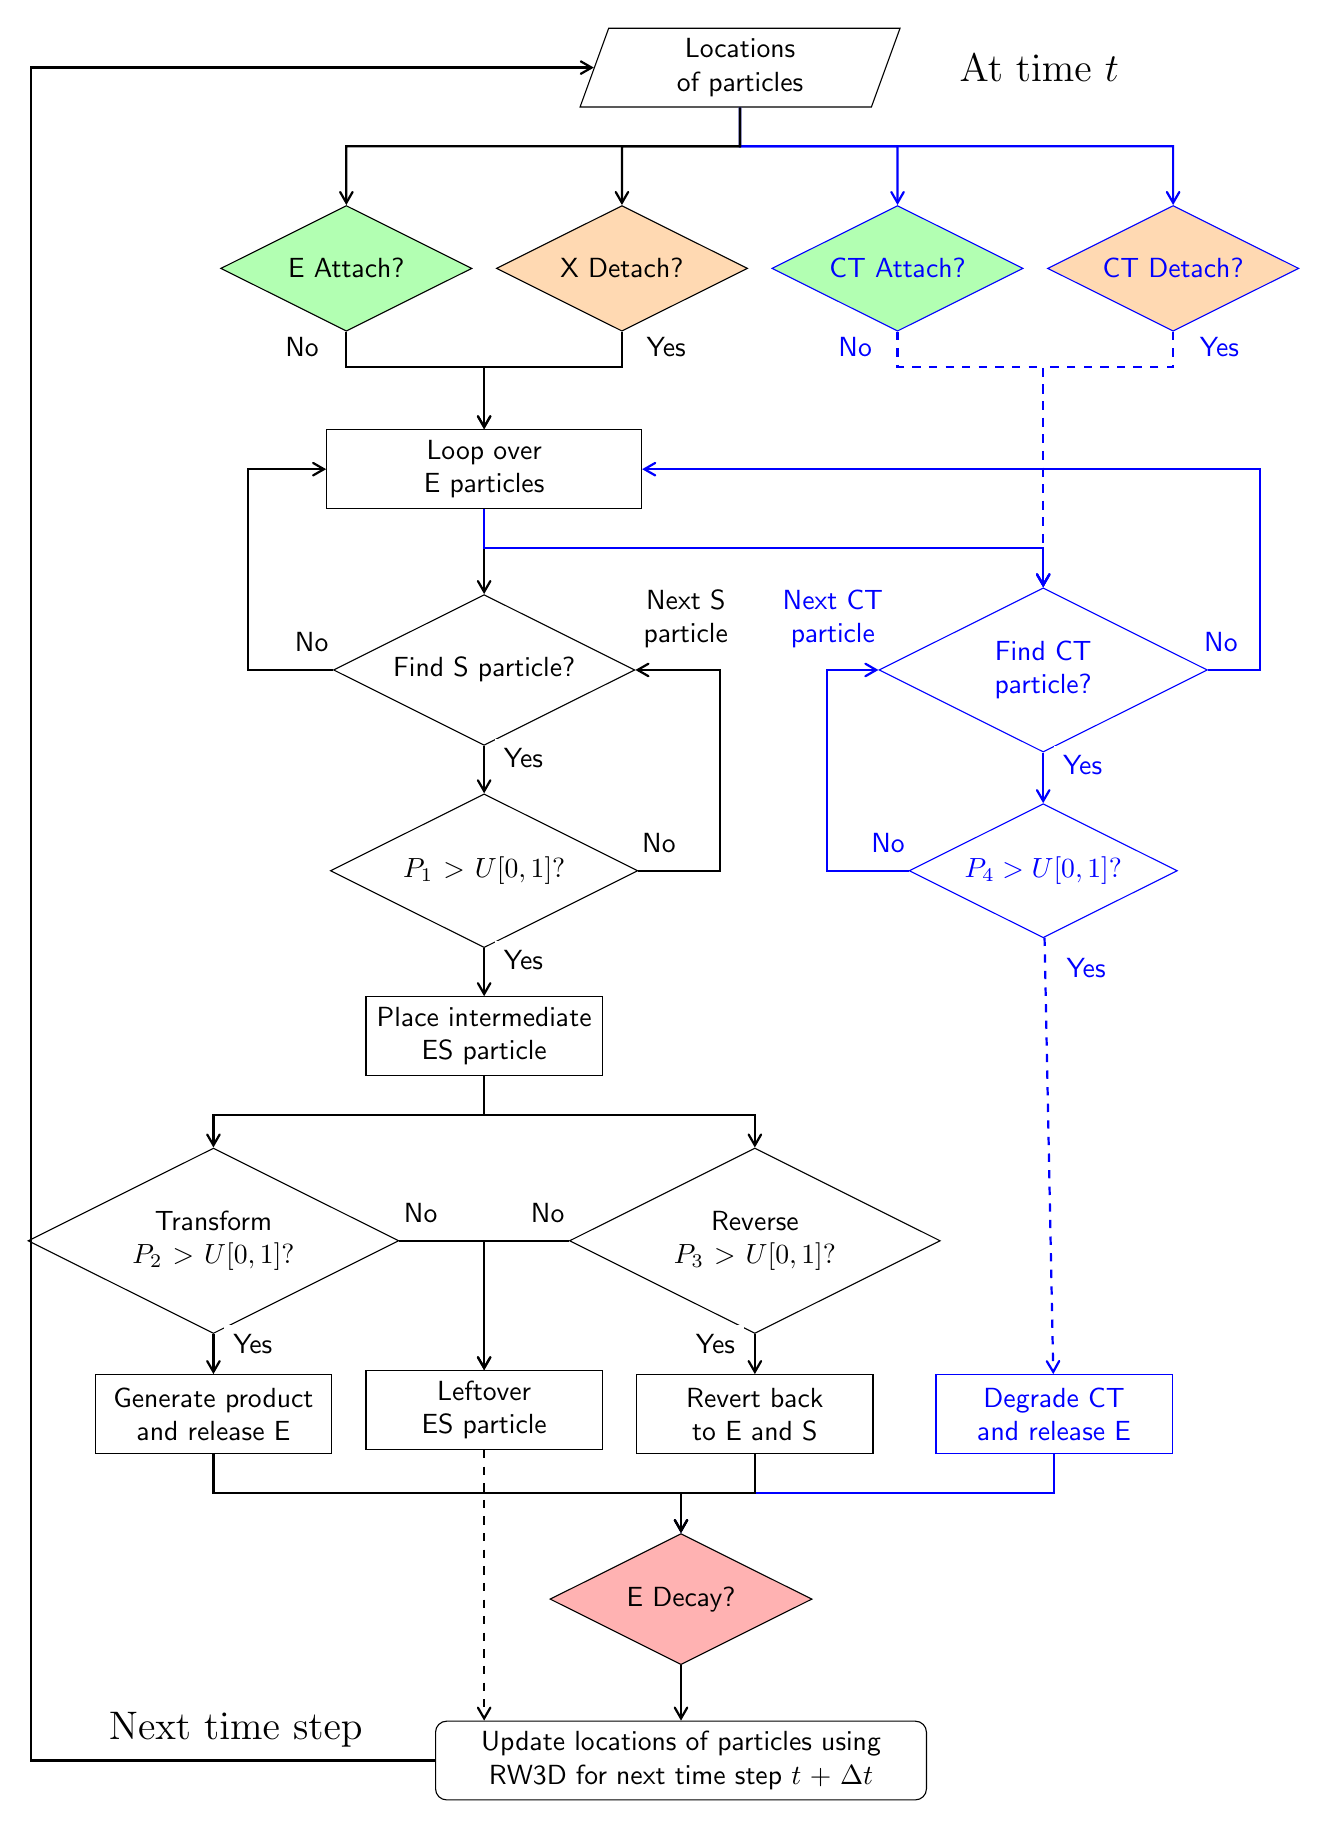
\begin{tikzpicture}[node distance=1.8cm,
    every node/.style={fill=white, font=\sffamily}, align=center]
  % Specification of nodes (position, etc.)

  \node (start_t)             [io_w]              {Locations of particles};
  \node (onatt_E)      [decision_s_g, below of=start_t, xshift = -5.cm, yshift=-0.75cm]   {E Attach?};
  \node (ondet_E)     [decision_s_o, below of=start_t, xshift = -1.5cm, yshift=-0.75cm]   {X Detach?};
  \node (onatt_c)      [decision_sb_g, below of=start_t, xshift =2. cm, yshift=-0.75cm]   {\color{blue} CT Attach?};
  \node (ondet_c)     [decision_sb_o, below of=start_t, xshift =5.5cm, yshift=-0.75cm]   {\color{blue} CT Detach?};
  \node (onLoop)     [process_w, below of=ondet_E, xshift = -1.75 cm, yshift=-0.75cm]          {Loop over E particles};
  \node (onSearch)      [decision, below of=onLoop, yshift=-0.75cm]   {Find S particle?};
  \node (onProb)     [decision, below of=onSearch, yshift=-0.75cm]   {$P_1>U[0,1]?$};
  \node (onIntermediate)      [process, below of=onProb, yshift=-0.3cm] {Place intermediate ES particle};
  \node (onTransform)      [decision, below left=1.5cm and 0.75cm of onIntermediate] 
                                                                {Transform $P_2>U[0,1]?$};
  \node (onReverse)      [decision, below right=1.5cm and 0.75 cm of onIntermediate] 
                                                                {Reverse $P_3>U[0,1]?$};
  \node (onProduct)       [process, below of=onTransform, yshift=-0.4cm]
                                                                 {Generate product and release E};
  \node (onRevert)       [process, below of=onReverse, yshift=-0.4cm]
                                                                 {Revert back to E and S};
 \node (onLeftover)       [process, below of =onIntermediate, yshift=-2.95cm]
                                                                 {Leftover ES particle};
  \node (onDecay)	 [decision_sr, below of=onLeftover, xshift = 2.5 cm, yshift=-0.6cm]
                                                    {E Decay?}; 
  \node (onNext)	 [Next, below of=onDecay, yshift=-0.25cm]
                                                    {Update locations of particles using RW3D for next time step $t + \Delta t$}; 

  \node (onSearch_CT)      [decision_b, right of=onSearch, xshift = 5.3 cm]   {\color{blue} Find CT particle?};
  \node (onProb_CT)     [decision_b, right of=onProb, xshift=5.3cm]   {\color{blue} $P_4>U[0,1]?$};
  \node (onDegrad)      [process_b, right of=onRevert, xshift=2.cm] {\color{blue} Degrade CT and release E};

  % Specification of lines between nodes specified above
  % with aditional nodes for description 
 % Specification of lines between nodes specified above
  % with aditional nodes for description 
 
 \draw[arrow2]		node[bignode, right of= start_t, xshift=2 cm] {At time $t$};
  %\draw[arrow2]		(start_t) -- (onLoop);

   \draw[arrow2b] 		(start_t)-- +(0,-1.) -| (onatt_c);
   \draw[arrow2b] 		(start_t)-- +(0,-1.) -| (ondet_c);
   \draw[arrow2] 		(start_t)-- +(0,-1.) -| (onatt_E);
   \draw[arrow2] 		(start_t)-- +(0,-1.) -| (ondet_E);

%   \draw[arrow2] 		([xshift=-5.5cm]start_t.south)-- (onatt_E);
%   \draw[arrow2] 		([xshift=-2.0cm]start_t.south)-- (ondet_E);
%   \draw[arrow2] 		([xshift=2.0cm]start_t.south)-- (onatt_c);
%   \draw[arrow2] 		([xshift=5.5cm]start_t.south)-- (ondet_c);

   \draw[arrow2] 		(onatt_E)-- +(0,-1.25) -| node [very near start, above, xshift = -1. cm, yshift=0. cm] {No} (onLoop);
   \draw[arrow2] 		(ondet_E)-- +(0,-1.25) -| node [very near start, above, xshift = 1. cm, yshift=0. cm] {Yes} (onLoop);

   \draw[arrow2bd] 		(onatt_c)-- +(0,-1.25) -| node [very near start, above, xshift = -1. cm, yshift=0. cm] {No} (onSearch_CT);
   \draw[arrow2bd] 		(ondet_c)-- +(0,-1.25) -| node [very near start, above, xshift = 1. cm, yshift=0. cm] {Yes} (onSearch_CT);

%   \draw[arrow2] 		(onatt_E)-- ([xshift=-5.5cm]onLoop.north);
%   \draw[arrow2] 		(ondet_E)-- ([xshift=-2.0cm]onLoop.north);

  %\draw[arrow2]		(onLoop) -- (onSearch);
   \draw[arrow2] 		(onLoop) -- +(0,-1.) -| (onSearch);
   \draw[arrow2b] 		(onLoop) -- +(0,-1.) -| (onSearch_CT);

  \draw[arrow2]		(onSearch) -- node [near start, xshift=0.5 cm]
                                {Yes} (onProb);
   \draw[arrow2] 		(onSearch)   --++  (-3.,0) node [near start, above, yshift=0.1 cm] {No} |- (onLoop);
   \draw[arrow2]		(onProb) -- node [near start, xshift=0.5 cm]
                                {Yes} (onIntermediate);
   \draw[arrow2]		(onProb)   --++  (3,0) node [near start, above, yshift=0.1 cm] {No} |- node [near end, above, text width=1.2 cm, xshift=0.1 cm, yshift=0.15 cm] {Next S particle} (onSearch);

   \draw[arrow2] 		(onIntermediate) -- +(0,-1.) -| (onTransform);
   \draw[arrow2] 		(onIntermediate) -- +(0,-1.) -| (onReverse);

  \draw[arrow2]		(onTransform) -- node [near start, xshift=0.5 cm]
                                {Yes} (onProduct);
   \draw[arrow2] 		(onTransform)   -| node [very near start, above, yshift=0.1 cm] {No} (onLeftover);

  \draw[arrow2]		(onReverse) -- node [near start, xshift=-0.5 cm]
                                {Yes} (onRevert);
   \draw[arrow2] 		(onReverse)   -| node [very near start, above, yshift=0.1 cm] {No} (onLeftover);

%  \draw[arrow2]             (onProduct) -- (onNext);
%  \draw[arrow2]             (onLeftover) -- (onNext);
%   \draw[arrow2]             (onRevert) -- (onNext);
 % \draw[->]             (onRevert) -- (onNext);

   \draw[arrow2b] 		(onDegrad) -- +(0,-1.) -| (onDecay);
   \draw[arrow2] 		(onProduct) -- +(0,-1.) -| (onDecay);
   \draw[arrow2] 		(onRevert) -- +(0,-1.) -| (onDecay);
   \draw[arrow2]               (onDecay) -- (onNext);
   \draw[arrow2] 		(onNext)   --++  (-8.25,0) node [bignode, near start, below, xshift=-1.25cm, yshift=0.75cm] {Next time step} |- (start_t);

   \draw[arrow2b] 		(onProb_CT)   --++  (-2.75,0) node [near start, above, yshift=0.1 cm] {No} |- node [near end, above, text width=1.5 cm, xshift=-0.25 cm, yshift=0.15 cm] {Next CT particle}(onSearch_CT);
 \draw[arrow2b]		(onSearch_CT)   --++  (2.75,0) node [near start, above, yshift=0.1 cm] {No} |- (onLoop);
\draw[arrow2b]		(onSearch_CT) -- node [near start, xshift=0.5 cm]
                                {Yes} (onProb_CT);
  \draw[arrow2bd]               (onProb_CT) -- node [near start, xshift=0.5 cm, yshift = 1.cm] {Yes} (onDegrad);
  \draw[arrow2d]             (onLeftover) -- ([xshift=-2.5cm]onNext.north);

\end{tikzpicture}
} %fbox
\end{document}

